
% Default to the notebook output style

    


% Inherit from the specified cell style.




    
\documentclass[11pt]{article}

    
    
    \usepackage[T1]{fontenc}
    % Nicer default font (+ math font) than Computer Modern for most use cases
    \usepackage{mathpazo}

    % Basic figure setup, for now with no caption control since it's done
    % automatically by Pandoc (which extracts ![](path) syntax from Markdown).
    \usepackage{graphicx}
    % We will generate all images so they have a width \maxwidth. This means
    % that they will get their normal width if they fit onto the page, but
    % are scaled down if they would overflow the margins.
    \makeatletter
    \def\maxwidth{\ifdim\Gin@nat@width>\linewidth\linewidth
    \else\Gin@nat@width\fi}
    \makeatother
    \let\Oldincludegraphics\includegraphics
    % Set max figure width to be 80% of text width, for now hardcoded.
    \renewcommand{\includegraphics}[1]{\Oldincludegraphics[width=.8\maxwidth]{#1}}
    % Ensure that by default, figures have no caption (until we provide a
    % proper Figure object with a Caption API and a way to capture that
    % in the conversion process - todo).
    \usepackage{caption}
    \DeclareCaptionLabelFormat{nolabel}{}
    \captionsetup{labelformat=nolabel}

    \usepackage{adjustbox} % Used to constrain images to a maximum size 
    \usepackage{xcolor} % Allow colors to be defined
    \usepackage{enumerate} % Needed for markdown enumerations to work
    \usepackage{geometry} % Used to adjust the document margins
    \usepackage{amsmath} % Equations
    \usepackage{amssymb} % Equations
    \usepackage{textcomp} % defines textquotesingle
    % Hack from http://tex.stackexchange.com/a/47451/13684:
    \AtBeginDocument{%
        \def\PYZsq{\textquotesingle}% Upright quotes in Pygmentized code
    }
    \usepackage{upquote} % Upright quotes for verbatim code
    \usepackage{eurosym} % defines \euro
    \usepackage[mathletters]{ucs} % Extended unicode (utf-8) support
    \usepackage[utf8x]{inputenc} % Allow utf-8 characters in the tex document
    \usepackage{fancyvrb} % verbatim replacement that allows latex
    \usepackage{grffile} % extends the file name processing of package graphics 
                         % to support a larger range 
    % The hyperref package gives us a pdf with properly built
    % internal navigation ('pdf bookmarks' for the table of contents,
    % internal cross-reference links, web links for URLs, etc.)
    \usepackage{hyperref}
    \usepackage{longtable} % longtable support required by pandoc >1.10
    \usepackage{booktabs}  % table support for pandoc > 1.12.2
    \usepackage[inline]{enumitem} % IRkernel/repr support (it uses the enumerate* environment)
    \usepackage[normalem]{ulem} % ulem is needed to support strikethroughs (\sout)
                                % normalem makes italics be italics, not underlines
    

    
    
    % Colors for the hyperref package
    \definecolor{urlcolor}{rgb}{0,.145,.698}
    \definecolor{linkcolor}{rgb}{.71,0.21,0.01}
    \definecolor{citecolor}{rgb}{.12,.54,.11}

    % ANSI colors
    \definecolor{ansi-black}{HTML}{3E424D}
    \definecolor{ansi-black-intense}{HTML}{282C36}
    \definecolor{ansi-red}{HTML}{E75C58}
    \definecolor{ansi-red-intense}{HTML}{B22B31}
    \definecolor{ansi-green}{HTML}{00A250}
    \definecolor{ansi-green-intense}{HTML}{007427}
    \definecolor{ansi-yellow}{HTML}{DDB62B}
    \definecolor{ansi-yellow-intense}{HTML}{B27D12}
    \definecolor{ansi-blue}{HTML}{208FFB}
    \definecolor{ansi-blue-intense}{HTML}{0065CA}
    \definecolor{ansi-magenta}{HTML}{D160C4}
    \definecolor{ansi-magenta-intense}{HTML}{A03196}
    \definecolor{ansi-cyan}{HTML}{60C6C8}
    \definecolor{ansi-cyan-intense}{HTML}{258F8F}
    \definecolor{ansi-white}{HTML}{C5C1B4}
    \definecolor{ansi-white-intense}{HTML}{A1A6B2}

    % commands and environments needed by pandoc snippets
    % extracted from the output of `pandoc -s`
    \providecommand{\tightlist}{%
      \setlength{\itemsep}{0pt}\setlength{\parskip}{0pt}}
    \DefineVerbatimEnvironment{Highlighting}{Verbatim}{commandchars=\\\{\}}
    % Add ',fontsize=\small' for more characters per line
    \newenvironment{Shaded}{}{}
    \newcommand{\KeywordTok}[1]{\textcolor[rgb]{0.00,0.44,0.13}{\textbf{{#1}}}}
    \newcommand{\DataTypeTok}[1]{\textcolor[rgb]{0.56,0.13,0.00}{{#1}}}
    \newcommand{\DecValTok}[1]{\textcolor[rgb]{0.25,0.63,0.44}{{#1}}}
    \newcommand{\BaseNTok}[1]{\textcolor[rgb]{0.25,0.63,0.44}{{#1}}}
    \newcommand{\FloatTok}[1]{\textcolor[rgb]{0.25,0.63,0.44}{{#1}}}
    \newcommand{\CharTok}[1]{\textcolor[rgb]{0.25,0.44,0.63}{{#1}}}
    \newcommand{\StringTok}[1]{\textcolor[rgb]{0.25,0.44,0.63}{{#1}}}
    \newcommand{\CommentTok}[1]{\textcolor[rgb]{0.38,0.63,0.69}{\textit{{#1}}}}
    \newcommand{\OtherTok}[1]{\textcolor[rgb]{0.00,0.44,0.13}{{#1}}}
    \newcommand{\AlertTok}[1]{\textcolor[rgb]{1.00,0.00,0.00}{\textbf{{#1}}}}
    \newcommand{\FunctionTok}[1]{\textcolor[rgb]{0.02,0.16,0.49}{{#1}}}
    \newcommand{\RegionMarkerTok}[1]{{#1}}
    \newcommand{\ErrorTok}[1]{\textcolor[rgb]{1.00,0.00,0.00}{\textbf{{#1}}}}
    \newcommand{\NormalTok}[1]{{#1}}
    
    % Additional commands for more recent versions of Pandoc
    \newcommand{\ConstantTok}[1]{\textcolor[rgb]{0.53,0.00,0.00}{{#1}}}
    \newcommand{\SpecialCharTok}[1]{\textcolor[rgb]{0.25,0.44,0.63}{{#1}}}
    \newcommand{\VerbatimStringTok}[1]{\textcolor[rgb]{0.25,0.44,0.63}{{#1}}}
    \newcommand{\SpecialStringTok}[1]{\textcolor[rgb]{0.73,0.40,0.53}{{#1}}}
    \newcommand{\ImportTok}[1]{{#1}}
    \newcommand{\DocumentationTok}[1]{\textcolor[rgb]{0.73,0.13,0.13}{\textit{{#1}}}}
    \newcommand{\AnnotationTok}[1]{\textcolor[rgb]{0.38,0.63,0.69}{\textbf{\textit{{#1}}}}}
    \newcommand{\CommentVarTok}[1]{\textcolor[rgb]{0.38,0.63,0.69}{\textbf{\textit{{#1}}}}}
    \newcommand{\VariableTok}[1]{\textcolor[rgb]{0.10,0.09,0.49}{{#1}}}
    \newcommand{\ControlFlowTok}[1]{\textcolor[rgb]{0.00,0.44,0.13}{\textbf{{#1}}}}
    \newcommand{\OperatorTok}[1]{\textcolor[rgb]{0.40,0.40,0.40}{{#1}}}
    \newcommand{\BuiltInTok}[1]{{#1}}
    \newcommand{\ExtensionTok}[1]{{#1}}
    \newcommand{\PreprocessorTok}[1]{\textcolor[rgb]{0.74,0.48,0.00}{{#1}}}
    \newcommand{\AttributeTok}[1]{\textcolor[rgb]{0.49,0.56,0.16}{{#1}}}
    \newcommand{\InformationTok}[1]{\textcolor[rgb]{0.38,0.63,0.69}{\textbf{\textit{{#1}}}}}
    \newcommand{\WarningTok}[1]{\textcolor[rgb]{0.38,0.63,0.69}{\textbf{\textit{{#1}}}}}
    
    
    % Define a nice break command that doesn't care if a line doesn't already
    % exist.
    \def\br{\hspace*{\fill} \\* }
    % Math Jax compatability definitions
    \def\gt{>}
    \def\lt{<}
    % Document parameters
    \title{AS A-Level Computer Science Projects}
    
    
    

    % Pygments definitions
    
\makeatletter
\def\PY@reset{\let\PY@it=\relax \let\PY@bf=\relax%
    \let\PY@ul=\relax \let\PY@tc=\relax%
    \let\PY@bc=\relax \let\PY@ff=\relax}
\def\PY@tok#1{\csname PY@tok@#1\endcsname}
\def\PY@toks#1+{\ifx\relax#1\empty\else%
    \PY@tok{#1}\expandafter\PY@toks\fi}
\def\PY@do#1{\PY@bc{\PY@tc{\PY@ul{%
    \PY@it{\PY@bf{\PY@ff{#1}}}}}}}
\def\PY#1#2{\PY@reset\PY@toks#1+\relax+\PY@do{#2}}

\expandafter\def\csname PY@tok@w\endcsname{\def\PY@tc##1{\textcolor[rgb]{0.73,0.73,0.73}{##1}}}
\expandafter\def\csname PY@tok@c\endcsname{\let\PY@it=\textit\def\PY@tc##1{\textcolor[rgb]{0.25,0.50,0.50}{##1}}}
\expandafter\def\csname PY@tok@cp\endcsname{\def\PY@tc##1{\textcolor[rgb]{0.74,0.48,0.00}{##1}}}
\expandafter\def\csname PY@tok@k\endcsname{\let\PY@bf=\textbf\def\PY@tc##1{\textcolor[rgb]{0.00,0.50,0.00}{##1}}}
\expandafter\def\csname PY@tok@kp\endcsname{\def\PY@tc##1{\textcolor[rgb]{0.00,0.50,0.00}{##1}}}
\expandafter\def\csname PY@tok@kt\endcsname{\def\PY@tc##1{\textcolor[rgb]{0.69,0.00,0.25}{##1}}}
\expandafter\def\csname PY@tok@o\endcsname{\def\PY@tc##1{\textcolor[rgb]{0.40,0.40,0.40}{##1}}}
\expandafter\def\csname PY@tok@ow\endcsname{\let\PY@bf=\textbf\def\PY@tc##1{\textcolor[rgb]{0.67,0.13,1.00}{##1}}}
\expandafter\def\csname PY@tok@nb\endcsname{\def\PY@tc##1{\textcolor[rgb]{0.00,0.50,0.00}{##1}}}
\expandafter\def\csname PY@tok@nf\endcsname{\def\PY@tc##1{\textcolor[rgb]{0.00,0.00,1.00}{##1}}}
\expandafter\def\csname PY@tok@nc\endcsname{\let\PY@bf=\textbf\def\PY@tc##1{\textcolor[rgb]{0.00,0.00,1.00}{##1}}}
\expandafter\def\csname PY@tok@nn\endcsname{\let\PY@bf=\textbf\def\PY@tc##1{\textcolor[rgb]{0.00,0.00,1.00}{##1}}}
\expandafter\def\csname PY@tok@ne\endcsname{\let\PY@bf=\textbf\def\PY@tc##1{\textcolor[rgb]{0.82,0.25,0.23}{##1}}}
\expandafter\def\csname PY@tok@nv\endcsname{\def\PY@tc##1{\textcolor[rgb]{0.10,0.09,0.49}{##1}}}
\expandafter\def\csname PY@tok@no\endcsname{\def\PY@tc##1{\textcolor[rgb]{0.53,0.00,0.00}{##1}}}
\expandafter\def\csname PY@tok@nl\endcsname{\def\PY@tc##1{\textcolor[rgb]{0.63,0.63,0.00}{##1}}}
\expandafter\def\csname PY@tok@ni\endcsname{\let\PY@bf=\textbf\def\PY@tc##1{\textcolor[rgb]{0.60,0.60,0.60}{##1}}}
\expandafter\def\csname PY@tok@na\endcsname{\def\PY@tc##1{\textcolor[rgb]{0.49,0.56,0.16}{##1}}}
\expandafter\def\csname PY@tok@nt\endcsname{\let\PY@bf=\textbf\def\PY@tc##1{\textcolor[rgb]{0.00,0.50,0.00}{##1}}}
\expandafter\def\csname PY@tok@nd\endcsname{\def\PY@tc##1{\textcolor[rgb]{0.67,0.13,1.00}{##1}}}
\expandafter\def\csname PY@tok@s\endcsname{\def\PY@tc##1{\textcolor[rgb]{0.73,0.13,0.13}{##1}}}
\expandafter\def\csname PY@tok@sd\endcsname{\let\PY@it=\textit\def\PY@tc##1{\textcolor[rgb]{0.73,0.13,0.13}{##1}}}
\expandafter\def\csname PY@tok@si\endcsname{\let\PY@bf=\textbf\def\PY@tc##1{\textcolor[rgb]{0.73,0.40,0.53}{##1}}}
\expandafter\def\csname PY@tok@se\endcsname{\let\PY@bf=\textbf\def\PY@tc##1{\textcolor[rgb]{0.73,0.40,0.13}{##1}}}
\expandafter\def\csname PY@tok@sr\endcsname{\def\PY@tc##1{\textcolor[rgb]{0.73,0.40,0.53}{##1}}}
\expandafter\def\csname PY@tok@ss\endcsname{\def\PY@tc##1{\textcolor[rgb]{0.10,0.09,0.49}{##1}}}
\expandafter\def\csname PY@tok@sx\endcsname{\def\PY@tc##1{\textcolor[rgb]{0.00,0.50,0.00}{##1}}}
\expandafter\def\csname PY@tok@m\endcsname{\def\PY@tc##1{\textcolor[rgb]{0.40,0.40,0.40}{##1}}}
\expandafter\def\csname PY@tok@gh\endcsname{\let\PY@bf=\textbf\def\PY@tc##1{\textcolor[rgb]{0.00,0.00,0.50}{##1}}}
\expandafter\def\csname PY@tok@gu\endcsname{\let\PY@bf=\textbf\def\PY@tc##1{\textcolor[rgb]{0.50,0.00,0.50}{##1}}}
\expandafter\def\csname PY@tok@gd\endcsname{\def\PY@tc##1{\textcolor[rgb]{0.63,0.00,0.00}{##1}}}
\expandafter\def\csname PY@tok@gi\endcsname{\def\PY@tc##1{\textcolor[rgb]{0.00,0.63,0.00}{##1}}}
\expandafter\def\csname PY@tok@gr\endcsname{\def\PY@tc##1{\textcolor[rgb]{1.00,0.00,0.00}{##1}}}
\expandafter\def\csname PY@tok@ge\endcsname{\let\PY@it=\textit}
\expandafter\def\csname PY@tok@gs\endcsname{\let\PY@bf=\textbf}
\expandafter\def\csname PY@tok@gp\endcsname{\let\PY@bf=\textbf\def\PY@tc##1{\textcolor[rgb]{0.00,0.00,0.50}{##1}}}
\expandafter\def\csname PY@tok@go\endcsname{\def\PY@tc##1{\textcolor[rgb]{0.53,0.53,0.53}{##1}}}
\expandafter\def\csname PY@tok@gt\endcsname{\def\PY@tc##1{\textcolor[rgb]{0.00,0.27,0.87}{##1}}}
\expandafter\def\csname PY@tok@err\endcsname{\def\PY@bc##1{\setlength{\fboxsep}{0pt}\fcolorbox[rgb]{1.00,0.00,0.00}{1,1,1}{\strut ##1}}}
\expandafter\def\csname PY@tok@kc\endcsname{\let\PY@bf=\textbf\def\PY@tc##1{\textcolor[rgb]{0.00,0.50,0.00}{##1}}}
\expandafter\def\csname PY@tok@kd\endcsname{\let\PY@bf=\textbf\def\PY@tc##1{\textcolor[rgb]{0.00,0.50,0.00}{##1}}}
\expandafter\def\csname PY@tok@kn\endcsname{\let\PY@bf=\textbf\def\PY@tc##1{\textcolor[rgb]{0.00,0.50,0.00}{##1}}}
\expandafter\def\csname PY@tok@kr\endcsname{\let\PY@bf=\textbf\def\PY@tc##1{\textcolor[rgb]{0.00,0.50,0.00}{##1}}}
\expandafter\def\csname PY@tok@bp\endcsname{\def\PY@tc##1{\textcolor[rgb]{0.00,0.50,0.00}{##1}}}
\expandafter\def\csname PY@tok@fm\endcsname{\def\PY@tc##1{\textcolor[rgb]{0.00,0.00,1.00}{##1}}}
\expandafter\def\csname PY@tok@vc\endcsname{\def\PY@tc##1{\textcolor[rgb]{0.10,0.09,0.49}{##1}}}
\expandafter\def\csname PY@tok@vg\endcsname{\def\PY@tc##1{\textcolor[rgb]{0.10,0.09,0.49}{##1}}}
\expandafter\def\csname PY@tok@vi\endcsname{\def\PY@tc##1{\textcolor[rgb]{0.10,0.09,0.49}{##1}}}
\expandafter\def\csname PY@tok@vm\endcsname{\def\PY@tc##1{\textcolor[rgb]{0.10,0.09,0.49}{##1}}}
\expandafter\def\csname PY@tok@sa\endcsname{\def\PY@tc##1{\textcolor[rgb]{0.73,0.13,0.13}{##1}}}
\expandafter\def\csname PY@tok@sb\endcsname{\def\PY@tc##1{\textcolor[rgb]{0.73,0.13,0.13}{##1}}}
\expandafter\def\csname PY@tok@sc\endcsname{\def\PY@tc##1{\textcolor[rgb]{0.73,0.13,0.13}{##1}}}
\expandafter\def\csname PY@tok@dl\endcsname{\def\PY@tc##1{\textcolor[rgb]{0.73,0.13,0.13}{##1}}}
\expandafter\def\csname PY@tok@s2\endcsname{\def\PY@tc##1{\textcolor[rgb]{0.73,0.13,0.13}{##1}}}
\expandafter\def\csname PY@tok@sh\endcsname{\def\PY@tc##1{\textcolor[rgb]{0.73,0.13,0.13}{##1}}}
\expandafter\def\csname PY@tok@s1\endcsname{\def\PY@tc##1{\textcolor[rgb]{0.73,0.13,0.13}{##1}}}
\expandafter\def\csname PY@tok@mb\endcsname{\def\PY@tc##1{\textcolor[rgb]{0.40,0.40,0.40}{##1}}}
\expandafter\def\csname PY@tok@mf\endcsname{\def\PY@tc##1{\textcolor[rgb]{0.40,0.40,0.40}{##1}}}
\expandafter\def\csname PY@tok@mh\endcsname{\def\PY@tc##1{\textcolor[rgb]{0.40,0.40,0.40}{##1}}}
\expandafter\def\csname PY@tok@mi\endcsname{\def\PY@tc##1{\textcolor[rgb]{0.40,0.40,0.40}{##1}}}
\expandafter\def\csname PY@tok@il\endcsname{\def\PY@tc##1{\textcolor[rgb]{0.40,0.40,0.40}{##1}}}
\expandafter\def\csname PY@tok@mo\endcsname{\def\PY@tc##1{\textcolor[rgb]{0.40,0.40,0.40}{##1}}}
\expandafter\def\csname PY@tok@ch\endcsname{\let\PY@it=\textit\def\PY@tc##1{\textcolor[rgb]{0.25,0.50,0.50}{##1}}}
\expandafter\def\csname PY@tok@cm\endcsname{\let\PY@it=\textit\def\PY@tc##1{\textcolor[rgb]{0.25,0.50,0.50}{##1}}}
\expandafter\def\csname PY@tok@cpf\endcsname{\let\PY@it=\textit\def\PY@tc##1{\textcolor[rgb]{0.25,0.50,0.50}{##1}}}
\expandafter\def\csname PY@tok@c1\endcsname{\let\PY@it=\textit\def\PY@tc##1{\textcolor[rgb]{0.25,0.50,0.50}{##1}}}
\expandafter\def\csname PY@tok@cs\endcsname{\let\PY@it=\textit\def\PY@tc##1{\textcolor[rgb]{0.25,0.50,0.50}{##1}}}

\def\PYZbs{\char`\\}
\def\PYZus{\char`\_}
\def\PYZob{\char`\{}
\def\PYZcb{\char`\}}
\def\PYZca{\char`\^}
\def\PYZam{\char`\&}
\def\PYZlt{\char`\<}
\def\PYZgt{\char`\>}
\def\PYZsh{\char`\#}
\def\PYZpc{\char`\%}
\def\PYZdl{\char`\$}
\def\PYZhy{\char`\-}
\def\PYZsq{\char`\'}
\def\PYZdq{\char`\"}
\def\PYZti{\char`\~}
% for compatibility with earlier versions
\def\PYZat{@}
\def\PYZlb{[}
\def\PYZrb{]}
\makeatother


    % Exact colors from NB
    \definecolor{incolor}{rgb}{0.0, 0.0, 0.5}
    \definecolor{outcolor}{rgb}{0.545, 0.0, 0.0}



    
    % Prevent overflowing lines due to hard-to-break entities
    \sloppy 
    % Setup hyperref package
    \hypersetup{
      breaklinks=true,  % so long urls are correctly broken across lines
      colorlinks=true,
      urlcolor=urlcolor,
      linkcolor=linkcolor,
      citecolor=citecolor,
      }
    % Slightly bigger margins than the latex defaults
    
    \geometry{verbose,tmargin=1in,bmargin=1in,lmargin=1in,rmargin=1in}
    
    

    \begin{document}
    
    
    \maketitle
    
    

    
    \section{AS / A Level OCR Computer
Science}\label{as-a-level-ocr-computer-science}

    \subsection{Introduction - Mini programming
projects}\label{introduction---mini-programming-projects}

    We aim to : 1. Use the OCR criteria project to design, analyse and
develop simple projects; 2. Identify mini-projects to help develop our
programming techniques; 3. Develop our skills at computational thinking:
decomposition and abstraction; 4. To develop real-world programming
problem solving: how do we find the parts of a problem to work on first?
5. Develop effective ways of working and research to solve our
self-defined programming problems. 6. Identify ways in which we can find
complexity in a project idea, following OCR

We spent some time identifying short projects to develop our skills.
This notebook summarises our steps and demonstrates the worked example
of the \textbf{Bingo} project. I try to expose how I think about solving
a programming problem and what drives my explorations and research. I
feel I am always learning and have built up a collection of research
techniques to aid my own learning.

    \subsection{OCR programming projects}\label{ocr-programming-projects}

    Use the following headings and prompt questions to structure your
thinking. Remember our discussion of what problems are \emph{computable}
or \emph{solvable by computational methods} (See PG Online OCR AS and A
Leveltextbook: page 277). Note that these are just the first few
statements, there are more points on \emph{development} and
\emph{evaluation}.

\textbf{Extract OCR A Level Computer Science Specification, pg.13-14}

\textbf{3.1 Analysis of the problem (10 marks)}

\textbar{}

Stages

\textbar{}

Prompts

\begin{longtable}[]{@{}lc@{}}
\toprule
\bottomrule
\end{longtable}

\textbar{}

3.1.1 Problem identification.

\begin{verbatim}
        | <p align="left">  (a) Describe and justify the features that make the problem solvable by computational methods. <br>(b) Explain why the problem is amenable to a computational approach.</p>     |
\end{verbatim}

\textbar{}

3.1.2 Stakeholders.

\begin{verbatim}
                 | <p align="left">  (a) Identify and describe those who will have an interest in the solution explaining how the solution is appropriate to their needs (this may be named individuals, groups or persona that describes the target end user).</p> |
\end{verbatim}

\textbar{}

3.1.3 Research the problem.

\textbar{}

\begin{enumerate}
\def\labelenumi{(\alph{enumi})}
\tightlist
\item
  Research the problem and solutions to similar problems to identify and
  justify suitable approaches to a solution.(b) Describe the essential
  features of a computational solution explaining these choices.(c)
  Explain the limitations of the proposed solution.

  \textbar{} \textbar{}

  3.1.4 Specify the proposed solution.

  \textbar{}

  \begin{enumerate}
  \def\labelenumii{(\alph{enumii})}
  \tightlist
  \item
    Specify and justify the solution requirements including hardware and
    software configuration (if appropriate).(b) Identify and justify
    measurable success criteria for the proposed solution.
  \end{enumerate}
\end{enumerate}

    \textbf{3.2 Design of the solution (15 marks)}

\textbar{}

Stages

\textbar{}

Prompts

\begin{longtable}[]{@{}lc@{}}
\toprule
\bottomrule
\end{longtable}

\textbar{}

3.2.1 Decompose the problem

\textbar{}

\begin{enumerate}
\def\labelenumi{(\alph{enumi})}
\tightlist
\item
  Break down the problem into smaller parts suitable for computational
  solutions justifying any decisions made.

  \textbar{} \textbar{}

  3.2.2 Describe the solution.

  \textbar{}

  \begin{enumerate}
  \def\labelenumii{(\alph{enumii})}
  \tightlist
  \item
    Explain and justify the structure of the solution. (b) Describe the
    parts of the solution using algorithms justifying how these
    algorithms form a complete solution to the problem.(c) Describe
    usability features to be included in the solution.(d) Identify key
    variables / data structures / classes justifying choices and any
    necessary validation.

    \textbar{} \textbar{}

    3.2.3 Describe the approach to testing. \textbar{}

    \begin{enumerate}
    \def\labelenumiii{(\alph{enumiii})}
    \tightlist
    \item
      Identify the test data to be used during the iterative development
      and post development phases and justify the choice of this test
      data.
    \end{enumerate}
  \end{enumerate}
\end{enumerate}

    \textbf{3.3 Developing the solution (25 marks)}

\textbar{}

Stages

\textbar{}

Prompts

\begin{longtable}[]{@{}lc@{}}
\toprule
\bottomrule
\end{longtable}

\textbar{}

3.3.1 Iterative development process

\textbar{}

\begin{enumerate}
\def\labelenumi{(\alph{enumi})}
\tightlist
\item
  Provide annotated evidence of each stage of the iterative development
  process justifying any decision made.(b) Provide annotated evidence of
  prototype solutions justifying any decision made.
\end{enumerate}

    \subsection{The iterative development
cycle}\label{the-iterative-development-cycle}

    You'll learn more about agile project management later. For our
mini-projects we want to do fast, iterative (cyclical) development. We
need to quickly \textbf{specify} our project, \textbf{identify} clear
sub-tasks that involve a concept we wish (or need) to know about, then
\textbf{research} and \textbf{develop} minimal working examples. In the
mini-projects we aim for a \emph{proof of concept}. The idea is to
collect a set of short, but complete programs that we can collect, use
as reference and, hopefully, assemble with little change into bigger
more complex project.

    \begin{figure}
\centering
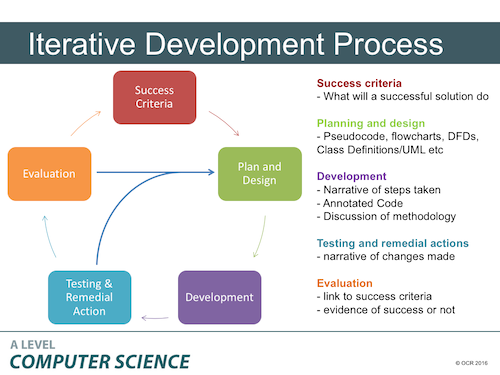
\includegraphics{OCR_A-Level_CS_Project_iterative_development_process.png}
\caption{OCR\_A-Level\_CS\_Project\_iterative\_development\_process.png}
\end{figure}

    \subsection{Set up a decent development
environment}\label{set-up-a-decent-development-environment}

    In the school computer lab, you need to install the latest Python
\url{https://www.python.org/downloads/} and install Portable VSCode
\url{https://sourceforge.net/projects/vscode-portable/}. Josh has an
excellent workflow to ensure he has a \emph{sane} development
environment whereever he goes. He carries it around on a USB.

Do this and you can install third party modules using pip.

    \subsection{Bingo!}\label{bingo}

    Tami, Stephanie and Adedolapo all suggested \textbf{Bingo} as a python
project, so I thought I'd help and have a go at identifying some of the
problems, identifying the python programming techniques we could explore
and writing some code. It is not a complete solution - instead I address
sub-problems that could be part of a bigger solution. Without getting
too detailed, I try and outline my thinking processes and research. I
also aim to explore some techniques that may help find \emph{complexity}
in the project: e.g. UI, data persistence (databases).

    \subsubsection{Research the rules of
bingo}\label{research-the-rules-of-bingo}

    \textbf{Web search:} I quickly identified UK and US bingo game rules and
found some interesting details about the construction of the bingo
cards.

UK bingo cards have 9 columns x 3 rows. There are 90 balls, selected at
random by a caller with a mechanical machine or a random number
generator. There are variations, but a player wins when a line is
matched or the whole card is matched. Game variations include matching
four corners. On the bingo card, each column is populated by random
numbers between 1 and 90, placed in a specific order in each column
(numeric value asc.) Column 1 contains numbers 1-10, column 2 11-20,
column three 21-30... and so on. Each row contains 4 blank squares. I
didn't realise there was such a rule-set and thought it would be fun to
try to code a card generator that obeyed the official UK Bingo rules.

\begin{figure}
\centering
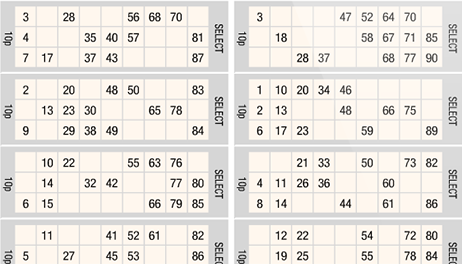
\includegraphics{OCR_A-Level_bingo_card.png}
\caption{OCR\_A-Level\_bingo\_card.png}
\end{figure}

There are many other variations of how bingo is played electronically:
against a computer, against others (networked), generate materials and
play offline (print out cards), and then many variations as to how the
game mechanics work.

I found another article
(\url{https://www.stat.berkeley.edu/~aldous/157/Old_Projects/chon.pdf})
interested in how the random distribution of numbers works
(statistically) and the problem of defining cards that limit the number
of winners in a game. I was surprised at the probability theory used to
analyse the problem. For now, as I did need to limit the number of cash
prizes (and the game isn't public), I would ignore the
business/ecomonics aspect of creating bingo cards. If I was coding an
online casino, I would care about this.

Just a quick survey made me think about the following:

\begin{enumerate}
\def\labelenumi{\arabic{enumi}.}
\tightlist
\item
  It is common to play multiple cards at once.
\item
  Online bingo systems often have real time chat facilities.
\item
  How do I handle random lists of numbers in Python?
\item
  How do I display tabulated content (like bingo cards in Python)
\item
  How do I store generated cards, in a database, for example?
\item
  How do I retrieve cards stored in a database?
\item
  How can I handle user interaction and events in Python and can I make
  an app with a GUI?
\item
  What is a suitable \emph{game mechanic} for bingo (written in Python)?
\end{enumerate}

Some small practical questions, and some bigger design questions.

Without much thought I jumped into coding and practically researching
Questions 3, 4 first, then 5, 6, then mayber 7.

Remember I am trying to test and extend my programming skills so these
seem like a good place to start.

    \subsubsection{Select a problem}\label{select-a-problem}

    \begin{itemize}
\tightlist
\item
  How do I handle random lists of numbers in Python?
\item
  How do I display tabulated content (like bingo cards in Python)
\item
  How do I store generated cards, in a database, for example?
\end{itemize}

Python can be extended using \emph{modules}. You may have seen:

import random

In a console python program, the print command doesn't print tables
nicely.

I had heard of the modules random, pprint and prettytables. I know about
lists. So I broke my problems down (decomposed them) into smaller bits
to help me refine my google searches.

The \href{https://docs.python.org/3/}{Python manual},
\href{https://stackoverflow.com}{Stackoverflow} and the git or home
pages of third party modules (e.g. for prettytable see
\url{https://code.google.com/archive/p/prettytable/wikis/Tutorial.wiki}
and \url{https://pypi.org/project/PrettyTable/} offer documentation and
code examples. Get used to reading documentation and examples,
extracting the bits you might need and try to build small working
programs that solve one problem.

    \subsubsection{Set up Python}\label{set-up-python}

    \textbf{Requirements:} I'm using the latest Python. And I can install
modules (python extensions) using:

pip install \textless{}module name\textgreater{}

    Install PrettyTable by running the following at your command line /
shell / powershell:

pip install PrettyTable

    If that doesn't work you may need to check your installation of python
(!).

    \subsubsection{Create your own development
environment}\label{create-your-own-development-environment}

    The school python installation is limited. You cannot install python
modules or extend python using pip install.

So: install your own:

\begin{enumerate}
\def\labelenumi{\arabic{enumi}.}
\tightlist
\item
  Download and install the latest python:
  \url{https://www.python.org/downloads/}
\item
  Download and install a good code editor (VS Code Portable):
  \url{https://sourceforge.net/projects/vscode-portable/}
\item
  Configure (Josh can explain).
\end{enumerate}

Then you are in control your coding environment on the school computers.

Josh carries his own \emph{sane} development environment around with him
on a USB. There are other ways to use a \emph{portable python} and
extend your environment.

\begin{enumerate}
\def\labelenumi{\arabic{enumi}.}
\tightlist
\item
  Use websites like \url{https://repl.it} or
  \url{https://www.pythonanywhere.com},
\item
  Use Docker containers \url{https://kitematic.com} - advanced;
\item
  Carry a
  \href{https://www.raspberrypi.org/documentation/usage/python/README.md}{Raspberry
  Pi} with you.
\end{enumerate}

    \subsubsection{Code - Pretty Table Random Bingo Card Test (with
comments)}\label{code---pretty-table-random-bingo-card-test-with-comments}

    The comments in the code below account my thought processes

    \begin{Verbatim}[commandchars=\\\{\}]
{\color{incolor}In [{\color{incolor}14}]:} \PY{k+kn}{from} \PY{n+nn}{prettytable} \PY{k}{import} \PY{n}{PrettyTable}
         \PY{k+kn}{from} \PY{n+nn}{prettytable} \PY{k}{import} \PY{n}{ALL} \PY{k}{as} \PY{n}{ALL} \PY{c+c1}{\PYZsh{} This was a nightmare to get working. I read the docs and looked for sample code. I tried about 10 attempts.}
         \PY{k+kn}{import} \PY{n+nn}{random}
         \PY{n}{bingoCard} \PY{o}{=} \PY{n}{PrettyTable}\PY{p}{(}\PY{n}{header} \PY{o}{=} \PY{k+kc}{False}\PY{p}{,} \PY{n}{hrules}\PY{o}{=}\PY{n}{ALL}\PY{p}{)} \PY{c+c1}{\PYZsh{} hrules: I really wanted to get lines between the rows! Took me ages.}
         \PY{n}{bingoCard}\PY{o}{.}\PY{n}{field\PYZus{}names} \PY{o}{=} \PY{p}{[}\PY{l+s+s1}{\PYZsq{}}\PY{l+s+s1}{Col1}\PY{l+s+s1}{\PYZsq{}}\PY{p}{,} \PY{l+s+s1}{\PYZsq{}}\PY{l+s+s1}{Col2}\PY{l+s+s1}{\PYZsq{}}\PY{p}{,} \PY{l+s+s1}{\PYZsq{}}\PY{l+s+s1}{Col3}\PY{l+s+s1}{\PYZsq{}}\PY{p}{,}\PY{l+s+s1}{\PYZsq{}}\PY{l+s+s1}{Col4}\PY{l+s+s1}{\PYZsq{}}\PY{p}{,}\PY{l+s+s1}{\PYZsq{}}\PY{l+s+s1}{Col5}\PY{l+s+s1}{\PYZsq{}}\PY{p}{,} \PY{l+s+s1}{\PYZsq{}}\PY{l+s+s1}{Col6}\PY{l+s+s1}{\PYZsq{}}\PY{p}{,} \PY{l+s+s1}{\PYZsq{}}\PY{l+s+s1}{Col7}\PY{l+s+s1}{\PYZsq{}}\PY{p}{,}\PY{l+s+s1}{\PYZsq{}}\PY{l+s+s1}{Col8}\PY{l+s+s1}{\PYZsq{}}\PY{p}{,}\PY{l+s+s1}{\PYZsq{}}\PY{l+s+s1}{Col9}\PY{l+s+s1}{\PYZsq{}}\PY{p}{]} \PY{c+c1}{\PYZsh{} set up headings to define the number of rows}
         
         \PY{n}{balls}\PY{o}{=}\PY{p}{[}\PY{p}{]} \PY{c+c1}{\PYZsh{} create an empty list}
         
         \PY{c+c1}{\PYZsh{} I never remember how range works. Look it up. I think I\PYZsq{}m getting numbers 1 \PYZhy{} 90 with no 0.}
         \PY{c+c1}{\PYZsh{} I thought of manually creating a list of numbers 1\PYZhy{}90 first. Then I thought of a for\PYZhy{}loop appending numbers}
         \PY{c+c1}{\PYZsh{} to an array/list. But python can do so much for you.}
         
         \PY{n}{balls} \PY{o}{=} \PY{n+nb}{list}\PY{p}{(}\PY{n+nb}{range}\PY{p}{(}\PY{l+m+mi}{1}\PY{p}{,}\PY{l+m+mi}{91}\PY{p}{)}\PY{p}{)} \PY{c+c1}{\PYZsh{} 90 balls in bingo \PYZhy{} no zero ball}
         
         \PY{c+c1}{\PYZsh{}some debug statements checking my list values, checking and demoing how random shuffle works. }
         \PY{c+c1}{\PYZsh{}I would remove these.}
         \PY{c+c1}{\PYZsh{}uncomment to see them working.}
         \PY{c+c1}{\PYZsh{}print(len(balls))}
         \PY{c+c1}{\PYZsh{}print(balls[89]) \PYZsh{} =90}
         \PY{c+c1}{\PYZsh{}print(balls[0]) \PYZsh{} =1}
         \PY{c+c1}{\PYZsh{}print(balls[90]) \PYZsh{} = index out of range error}
         \PY{c+c1}{\PYZsh{}random.shuffle(balls) \PYZsh{} run this every time you wish to shuffle the array. }
         
         \PY{c+c1}{\PYZsh{} I think I want to store the cards, before a reshuffle. Note check how to do this}
         
         \PY{c+c1}{\PYZsh{}print(balls[50])}
         \PY{c+c1}{\PYZsh{}random.shuffle(balls) \PYZsh{} uncomment to test that shuffle really does mix things up.}
         \PY{c+c1}{\PYZsh{}print(balls[50])}
         
         \PY{c+c1}{\PYZsh{} After a shuffle, I decided to use the first 27 items from the list. They should be random.}
         \PY{c+c1}{\PYZsh{} I prepare them in rows for prettytable}
         \PY{c+c1}{\PYZsh{} I adapted this sequence from the pretty table documentation. When you have a prettytable object, you can :}
         \PY{c+c1}{\PYZsh{}      * sort rows}
         \PY{c+c1}{\PYZsh{}      * add data in columns, not only rows (like here)}
         \PY{c+c1}{\PYZsh{}      * read and print a table from a database (e.g. sqlite)}
         \PY{c+c1}{\PYZsh{}      * change the formatting of the output table}
         \PY{c+c1}{\PYZsh{}      * print the table to HTML (this will be useful I feel)}
         
         \PY{c+c1}{\PYZsh{} There may be a better way to do this with for\PYZhy{}loops. Do it the long way (if it works). Optimise later.}
         \PY{n}{row1} \PY{o}{=} \PY{p}{[}\PY{n}{balls}\PY{p}{[}\PY{l+m+mi}{1}\PY{p}{]}\PY{p}{,} \PY{n}{balls}\PY{p}{[}\PY{l+m+mi}{2}\PY{p}{]}\PY{p}{,}  \PY{n}{balls}\PY{p}{[}\PY{l+m+mi}{3}\PY{p}{]}\PY{p}{,}  \PY{n}{balls}\PY{p}{[}\PY{l+m+mi}{4}\PY{p}{]}\PY{p}{,}  \PY{n}{balls}\PY{p}{[}\PY{l+m+mi}{5}\PY{p}{]}\PY{p}{,}  \PY{n}{balls}\PY{p}{[}\PY{l+m+mi}{6}\PY{p}{]}\PY{p}{,}  \PY{n}{balls}\PY{p}{[}\PY{l+m+mi}{7}\PY{p}{]}\PY{p}{,}  \PY{n}{balls}\PY{p}{[}\PY{l+m+mi}{8}\PY{p}{]}\PY{p}{,}  \PY{n}{balls}\PY{p}{[}\PY{l+m+mi}{9}\PY{p}{]}\PY{p}{]}
         \PY{n}{row2} \PY{o}{=} \PY{p}{[}\PY{n}{balls}\PY{p}{[}\PY{l+m+mi}{11}\PY{p}{]}\PY{p}{,}\PY{n}{balls}\PY{p}{[}\PY{l+m+mi}{12}\PY{p}{]}\PY{p}{,} \PY{n}{balls}\PY{p}{[}\PY{l+m+mi}{13}\PY{p}{]}\PY{p}{,} \PY{n}{balls}\PY{p}{[}\PY{l+m+mi}{14}\PY{p}{]}\PY{p}{,} \PY{n}{balls}\PY{p}{[}\PY{l+m+mi}{15}\PY{p}{]}\PY{p}{,} \PY{n}{balls}\PY{p}{[}\PY{l+m+mi}{16}\PY{p}{]}\PY{p}{,} \PY{n}{balls}\PY{p}{[}\PY{l+m+mi}{17}\PY{p}{]}\PY{p}{,} \PY{n}{balls}\PY{p}{[}\PY{l+m+mi}{18}\PY{p}{]}\PY{p}{,} \PY{n}{balls}\PY{p}{[}\PY{l+m+mi}{19}\PY{p}{]}\PY{p}{]}
         \PY{n}{row3} \PY{o}{=} \PY{p}{[}\PY{n}{balls}\PY{p}{[}\PY{l+m+mi}{20}\PY{p}{]}\PY{p}{,}\PY{n}{balls}\PY{p}{[}\PY{l+m+mi}{21}\PY{p}{]}\PY{p}{,} \PY{n}{balls}\PY{p}{[}\PY{l+m+mi}{22}\PY{p}{]}\PY{p}{,} \PY{n}{balls}\PY{p}{[}\PY{l+m+mi}{23}\PY{p}{]}\PY{p}{,} \PY{n}{balls}\PY{p}{[}\PY{l+m+mi}{24}\PY{p}{]}\PY{p}{,} \PY{n}{balls}\PY{p}{[}\PY{l+m+mi}{25}\PY{p}{]}\PY{p}{,} \PY{n}{balls}\PY{p}{[}\PY{l+m+mi}{26}\PY{p}{]}\PY{p}{,} \PY{n}{balls}\PY{p}{[}\PY{l+m+mi}{27}\PY{p}{]}\PY{p}{,}  \PY{n}{balls}\PY{p}{[}\PY{l+m+mi}{28}\PY{p}{]}\PY{p}{]}
         
         
         \PY{n}{bingoCard}\PY{o}{.}\PY{n}{add\PYZus{}row}\PY{p}{(}\PY{n}{row1}\PY{p}{)}
         \PY{n}{bingoCard}\PY{o}{.}\PY{n}{add\PYZus{}row}\PY{p}{(}\PY{n}{row2}\PY{p}{)}
         \PY{n}{bingoCard}\PY{o}{.}\PY{n}{add\PYZus{}row}\PY{p}{(}\PY{n}{row3}\PY{p}{)}
         
         \PY{n+nb}{print}\PY{p}{(}\PY{l+s+s2}{\PYZdq{}}\PY{l+s+s2}{Bingo Card}\PY{l+s+s2}{\PYZdq{}}\PY{p}{)}
         \PY{n+nb}{print} \PY{p}{(}\PY{n}{bingoCard}\PY{p}{)}
         \PY{c+c1}{\PYZsh{} Yay!}
\end{Verbatim}


    \begin{Verbatim}[commandchars=\\\{\}]
Bingo Card
+----+----+----+----+----+----+----+----+----+
| 2  | 3  | 4  | 5  | 6  | 7  | 8  | 9  | 10 |
+----+----+----+----+----+----+----+----+----+
| 12 | 13 | 14 | 15 | 16 | 17 | 18 | 19 | 20 |
+----+----+----+----+----+----+----+----+----+
| 21 | 22 | 23 | 24 | 25 | 26 | 27 | 28 | 29 |
+----+----+----+----+----+----+----+----+----+

    \end{Verbatim}

    \subsubsection{Research -}\label{research--}

    \subsection{Resources}\label{resources}

    OCR A Level Computer Science Specification
\url{http://www.ocr.org.uk/Images/170844-specification-accredited-a-level-gce-computer-science-h446.pdf}
See pages: 13-14

OCR A Level Computer Science Project Complexity Guide
\url{http://www.ocr.org.uk/Images/253701-project-complexity-guide.pdf}

OCR A Level Computer Science Project Teacher Guide
\url{http://www.ocr.org.uk/Images/324587-component-03-programming-project-teacher-guide.ppt}

Carroll, John and David Morris. 2017.
\emph{\href{http://ineasysteps.com/products-page/all_books/agile-project-management-easy-steps-2nd-edition/}{Agile
Project Management in easy steps}}. Lymington Spa, Easy Steps.


    % Add a bibliography block to the postdoc
    
    
    
    \end{document}
